\documentclass{article}

% ———————————————————————————————————————————————————————
%  PACKAGES (1 seule fois chacun)
% ———————————————————————————————————————————————————————
\usepackage{geometry}
\geometry{a4paper,left=0.6cm,right=0.7cm,top=1cm,bottom=1cm,columnsep=0.8cm}

\usepackage{times}
\usepackage{paracol}
\usepackage{enumitem}
\usepackage{fontawesome}
\usepackage{tabularx}
\usepackage{tikz}
\usepackage{adjustbox}
\usepackage[hidelinks]{hyperref}
\usepackage{xcolor}
\usepackage{ragged2e}

\setlist[itemize]{itemsep=2pt,topsep=0pt,leftmargin=*}
\renewcommand{\labelitemi}{\textcolor{maincolor}{$\bullet$}}

\newcolumntype{Y}{>{\RaggedRight\arraybackslash}X}
\setlength{\parindent}{0pt}

% ———————————————————————————————————————————————————————
%  COULEURS & MISE EN PAGE
% ———————————————————————————————————————————————————————
\definecolor{maincolor}{HTML}{f0fafc}
\definecolor{seccolor}{HTML}{ffffff}
\definecolor{gray}{HTML}{8c94a9}
\definecolor{sidetext}{HTML}{59cee5}


% bande colorée à droite
\usepackage{eso-pic}
\AddToShipoutPictureBG{%
  \begin{tikzpicture}[remember picture,overlay]
    \fill[maincolor!10] (0.7\paperwidth,0) rectangle (\paperwidth,\paperheight);
  \end{tikzpicture}
}

% en-tête de section compact
\newcommand{\cvsection}[1]{%
  \par\bigskip
  {\Large\bfseries #1}\par
  \noindent\rule{\linewidth}{0.6pt}\par
  \medskip
}

% ———————————————————————————————————————————————————————
%  DOCUMENT
% ———————————————————————————————————————————————————————
\begin{document}\pagestyle{empty}
\columnratio{0.7}\begin{paracol}{2}

% ========== Colonne principale ====================================
{\LARGE\bfseries Judikael Mourouvin}

{\color{maincolor}\Large\bfseries Technicien informatique \& marketing digital}

\medskip
%----------- contact résumé ----------------------------------------
\begin{tabular}{@{}cp{0.45\linewidth}}
  \color{maincolor}\faEnvelope & \href{mailto:jkmou971@gmail.com}{jkmou971@gmail.com}\\
  \color{maincolor}\faPhone    &  {+590 690 91 14 48}\\
  \color{maincolor}\faMapMarker& Route de COCOYER\\ 97190 GOSIER\\
  \color{maincolor}\faLinkedin & \href{}{}\\
\end{tabular}

\cvsection{PROFIL}
Passionné par l’informatique et le marketing digital, j’ai développé une solide expérience en configuration de postes, maintenance et diagnostic d’incidents. Mon année d’alternance à la DSI de la Mairie du Gosier m’a permis de mener des projets numériques et d’accompagner les utilisateurs au quotidien. Rigoureux et orienté résultat, je souhaite désormais mettre mes compétences au service d’une équipe dynamique à temps plein.

\cvsection{EXPÉRIENCE}

\colorbox{maincolor}{%
  \begin{minipage}{\linewidth}
    \textbf{Alternant en Marketing Digital} \\ Mairie du Gosier – DSI \\ 2023-2024
    \begin{itemize}
      \item Piloté des projets numériques municipaux, garantissant leur déploiement réussi \item Analysé les besoins des usagers et proposé des solutions adaptées \item Assuré support et formation, améliorant la maîtrise des outils digitaux
    \end{itemize}
  \end{minipage}}

\vspace{3mm}


\colorbox{maincolor}{%
  \begin{minipage}{\linewidth}
    \textbf{Animateur de la zone informatique} \\ Pôle Emploi, Gosier \\ 2022-2023
    \begin{itemize}
      \item Fournit un support technique quotidien aux demandeurs d’emploi \item Configuré et maintenu les postes de travail pour une disponibilité optimale \item Diagnostic des incidents et résolution rapide pour limiter les interruptions
    \end{itemize}
  \end{minipage}}

\vspace{3mm}


\colorbox{maincolor}{%
  \begin{minipage}{\linewidth}
    \textbf{Stagiaire Informaticien} \\ NUMERIKA, Baie Mahault \\ 2020-2021
    \begin{itemize}
      \item Installé et configuré équipements informatiques en environnement PME \item Réalisé la maintenance préventive et corrective du parc matériel \item Apporté un support de proximité aux utilisateurs internes
    \end{itemize}
  \end{minipage}}   %← généré par build_placeholders()

\cvsection{FORMATION}

    \begin{tabularx}{\linewidth}{@{}c X@{}}
    \textcolor{sidetext}{\faGraduationCap} &
    \textbf{Bachelor Marketing Digital} \\
    & CFA IUTS \\
    & \begin{itemize}[leftmargin=*]
  \item Stratégies de communication en ligne et gestion de contenu \item Analyse de données web et optimisation de campagnes numériques \item Gestion de projets digitaux et outils marketing
\end{itemize} \\
    & \textit{2023-2024}
    \end{tabularx}
    

\vspace{3mm}


    \begin{tabularx}{\linewidth}{@{}c X@{}}
    \textcolor{sidetext}{\faGraduationCap} &
    \textbf{BTS Système Numérique option Informatique et Réseaux} \\
    & Lycée de Chevalier Saint Georges, Abymes \\
    & \begin{itemize}[leftmargin=*]
  \item Architecture des réseaux et administration de systèmes \item Maintenance matérielle et logicielle de postes et serveurs \item Assistance technique et support utilisateur
\end{itemize} \\
    & \textit{2019-2021}
    \end{tabularx}
    

% ———— Colonne de droite (bleue) ————————————————
\switchcolumn
\color{black}           % le fond est déjà maincolor!10

\centering
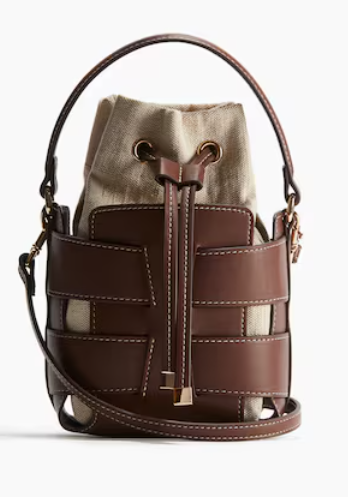
\includegraphics[width=3cm]{e75c7485d22d44e69e6d322ec66326d0.png}

\bigskip

\cvsection{COMPÉTENCES}

\begin{itemize}[leftmargin=*]
\item Administration
\item Réseaux
\item Support
\item Maintenance
\item Configuration
\item Marketing
\item Digital\end{itemize}


\cvsection{LANGUES}

\begin{itemize}[leftmargin=*]
\item English - \textcolor{gray}{}
\item Espagnol - \textcolor{gray}{}\end{itemize}


\cvsection{CENTRES D’INTÉRÊT}

\begin{itemize}[leftmargin=*]
\item Lecture \& veille technologique
\item Randonnée / sports outdoor
\item Voyages \& découverte culturelle
\end{itemize}


\end{paracol}
\end{document}
